\documentclass[10pt,aspectratio=169,serif]{beamer}

\usepackage[fontset=none, scheme=plain]{ctex}
\IfFontExistsTF{Songti SC}{%
	\setCJKmainfont{Songti SC}[AutoFakeSlant=0.2]%
	\setCJKsansfont{Songti SC}[AutoFakeSlant=0.2]%
}{%
	\setCJKmainfont{FandolSong-Regular}[Extension=.otf,BoldFont=FandolSong-Bold,AutoFakeSlant=0.2]%
	\setCJKsansfont{FandolSong-Regular}[Extension=.otf,BoldFont=FandolSong-Bold]%
}
\usepackage{amsmath,amssymb,graphicx,tikz,booktabs,multicol,calligra}
\usepackage{pgfplots}
\pgfplotsset{compat=1.18}
\usepackage{tcolorbox}
\tcbuselibrary{skins}
\usepackage{XyygU}
\usepackage{caption}
\captionsetup[figure]{name=图,labelsep=period}

\usetikzlibrary{arrows.meta,positioning,calc}

\setlength{\abovedisplayskip}{0pt plus 2pt minus 2pt}
\setlength{\belowdisplayskip}{0pt plus 2pt minus 2pt}

\title[三角函数图象与性质练习]{5.4 三角函数的图象与性质（练习）}
\subtitle{正弦、余弦曲线 \& 性质 \& 正切曲线}
\author{}
\institute{}
\date{2026-10-16}

\begin{document}

\begin{frame}
  \titlepage
\end{frame}

% ==================================================================
\section*{练习（一）正弦函数、余弦函数的图象}
% ==================================================================

% ---------- 第1题 ----------
\begin{frame}[t]{练习一 1：画正弦、余弦曲线并比较异同}
\textbf{1.} 在同一直角坐标系中，画出函数
\[
y=\sin x,\ x\in[0,2\pi],\qquad y=\cos x,\ x\in\!\left[-\frac{\pi}{2},\frac{3\pi}{2}\right]
\]
的图象。通过观察两条曲线，说出它们的异同。
\end{frame}

\begin{frame}[t]{练习一 1 图象}
\begin{center}
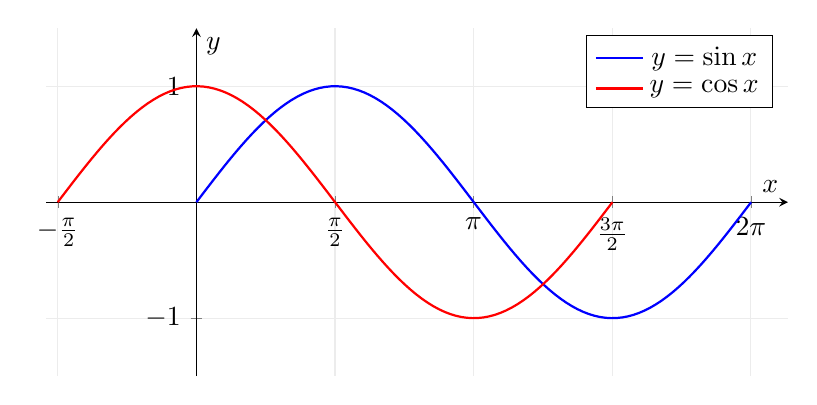
\begin{tikzpicture}
\begin{axis}[
    width=11cm, height=6cm,
    axis lines=middle,
    xlabel={$x$}, ylabel={$y$},
    xmin=-1.7, xmax=6.7, ymin=-1.5, ymax=1.5,
    xtick={-1.57,0,1.57,3.14,4.71,6.28},
    xticklabels={$-\frac\pi2$,$0$,$\frac\pi2$,$\pi$,$\frac{3\pi}{2}$,$2\pi$},
    ytick={-1,1},
    grid=major, grid style={gray!15},
]
\addplot[thick,blue,domain=0:6.283,samples=100] {sin(deg(x))};
\addlegendentry{$y=\sin x$}
\addplot[thick,red,domain=-1.571:4.712,samples=100] {cos(deg(x))};
\addlegendentry{$y=\cos x$}
\end{axis}
\end{tikzpicture}
\end{center}
\end{frame}

\begin{frame}[t]{练习一 1 解答}
\begin{tcolorbox}[colback=orange!10,colframe=orange,title=\textbf{异同}]
\textbf{相同点：}
\begin{itemize}
  \item 形状完全相同，都是“波浪起伏”的连续光滑曲线；
  \item 周期都是 $2\pi$，值域都是 $[-1,1]$；
  \item 都在 $[-1,1]$ 上振荡，有最大值 $1$、最小值 $-1$。
\end{itemize}
\textbf{不同点：}
\begin{itemize}
  \item 位置不同：余弦曲线可由正弦曲线\alert{向左平移 $\dfrac{\pi}{2}$ 个单位}得到，即
  \[
  \cos x=\sin\!\left(x+\frac{\pi}{2}\right).
  \]
  \item 与坐标轴的交点、最值点位置不同。
\end{itemize}
\end{tcolorbox}
\end{frame}

% ---------- 第2题 ----------
\begin{frame}[t]{练习一 2：五点法作图}
\textbf{2.} 用五点法分别画下列函数在 $[-\pi,\pi]$ 上的图象：
\begin{enumerate}[(1)]
  \item $y=-\sin x$； \qquad
  \item $y=2-\cos x$。
\end{enumerate}
\vspace{0.5em}
\small 五点：取 $x=-\pi,-\dfrac{\pi}{2},0,\dfrac{\pi}{2},\pi$。
\end{frame}

\begin{frame}[t]{练习一 2 解答与图象}
\begin{columns}
\begin{column}{0.48\textwidth}
\small
\begin{tabular}{c|ccccc}
$x$ & $-\pi$ & $-\frac\pi2$ & $0$ & $\frac\pi2$ & $\pi$\\
\hline
$\sin x$ & $0$ & $-1$ & $0$ & $1$ & $0$\\
$-\sin x$ & $0$ & $1$ & $0$ & $-1$ & $0$\\
\hline
$\cos x$ & $-1$ & $0$ & $1$ & $0$ & $-1$\\
$2-\cos x$ & $3$ & $2$ & $1$ & $2$ & $3$\\
\end{tabular}
\end{column}
\begin{column}{0.52\textwidth}
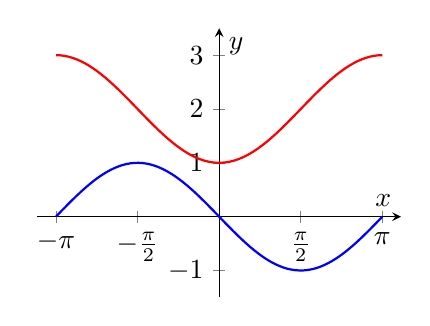
\begin{tikzpicture}
\begin{axis}[
    width=6.2cm, height=5cm,
    axis lines=middle,
    xlabel={$x$}, ylabel={$y$},
    xmin=-3.5, xmax=3.5, ymin=-1.5, ymax=3.5,
    xtick={-3.14,-1.57,0,1.57,3.14},
    xticklabels={$-\pi$,$-\frac\pi2$,$0$,$\frac\pi2$,$\pi$},
    ytick={-1,1,2,3},
]
\addplot[thick,blue,domain=-3.14:3.14,samples=80] {-sin(deg(x))};
\addplot[thick,red,domain=-3.14:3.14,samples=80] {2-cos(deg(x))};
\end{axis}
\end{tikzpicture}
\end{column}
\end{columns}
\end{frame}

% ---------- 第3题 ----------
\begin{frame}[t]{练习一 3：$y=|\sin x|$ 的图象}
\textbf{3.} 想一想函数 $y=|\sin x|$ 与 $y=\sin x$ 的图象及其关系，并借助信息技术画出函数的图象进行检验。
\end{frame}

\begin{frame}[t]{练习一 3 解答}
\begin{columns}
\begin{column}{0.55\textwidth}
\begin{tcolorbox}[colback=orange!10,colframe=orange,title=\textbf{解}]
\begin{itemize}
  \item $y=|\sin x|$ 是把 $y=\sin x$ 图象中\alert{$x$ 轴下方的部分沿 $x$ 轴翻折到上方}；
  \item 值域由 $[-1,1]$ 变为 $[0,1]$；
  \item 周期由 $2\pi$ 变为 $\pi$；
  \item $|\sin(x+\pi)|=|-\sin x|=|\sin x|$。
\end{itemize}
\end{tcolorbox}
\end{column}
\begin{column}{0.45\textwidth}
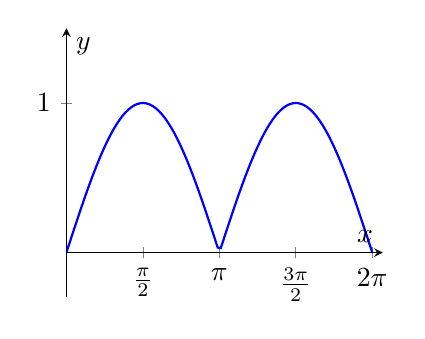
\begin{tikzpicture}
\begin{axis}[
    width=5.6cm, height=5cm,
    axis lines=middle,
    xlabel={$x$}, ylabel={$y$},
    xmin=0, xmax=6.5, ymin=-0.3, ymax=1.5,
    xtick={1.57,3.14,4.71,6.28},
    xticklabels={$\frac\pi2$,$\pi$,$\frac{3\pi}{2}$,$2\pi$},
    ytick={0,1},
]
\addplot[thick,blue,domain=0:6.28,samples=100] {abs(sin(deg(x)))};
\end{axis}
\end{tikzpicture}
\end{column}
\end{columns}
\end{frame}

% ---------- 第4题 ----------
\begin{frame}[t]{练习一 4：多项选择}
\textbf{4.}（多项选择题）函数 $y=1+\cos x$，$x\in\!\left(\dfrac{\pi}{3},2\pi\right)$ 的图象与直线 $y=t$（$t$ 为常数）的交点可能有（\quad ）。

\vspace{1em}
\begin{columns}
\begin{column}{0.2\textwidth}{(A) 0 个}\end{column}
\begin{column}{0.2\textwidth}{(B) 1 个}\end{column}
\begin{column}{0.2\textwidth}{(C) 2 个}\end{column}
\begin{column}{0.2\textwidth}{(D) 3 个}\end{column}
\begin{column}{0.2\textwidth}{(E) 4 个}\end{column}
\end{columns}
\end{frame}

\begin{frame}[t]{练习一 4 解答}
\begin{columns}
\begin{column}{0.55\textwidth}
\begin{tcolorbox}[colback=orange!10,colframe=orange,title=\textbf{解}]
在 $\left(\dfrac{\pi}{3},2\pi\right)$ 上：
$y=1+\cos x$ 从 $1+\dfrac12=\dfrac32$（$x=\dfrac\pi3$，开区间）递减到 $0$（$x=\pi$），再递增到 $2$（$x=2\pi$，开区间）。
\vspace{0.3em}
\begin{itemize}
  \item $t<0$ 或 $t\ge 2$：\alert{0 个}交点；
  \item $t=0$：在 $x=\pi$ 处 \alert{1 个}交点；
  \item $0<t<\dfrac32$：左右各 $1$ 个，共 \alert{2 个}；
  \item $\dfrac32\le t<2$：右侧 $1$ 个，共 \alert{1 个}。
\end{itemize}
故交点个数可能为 $0,1,2$。选 \alert{(A)(B)(C)}。
\end{tcolorbox}
\end{column}
\begin{column}{0.45\textwidth}
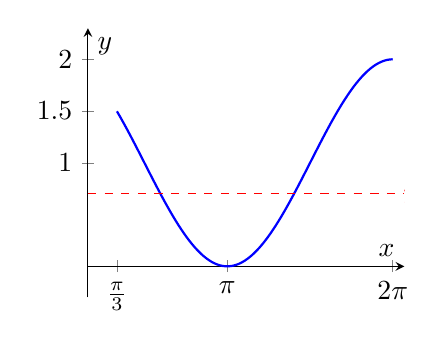
\begin{tikzpicture}
\begin{axis}[
    width=5.6cm, height=5cm,
    axis lines=middle,
    xlabel={$x$}, ylabel={$y$},
    xmin=0.5, xmax=6.5, ymin=-0.3, ymax=2.3,
    xtick={1.05,3.14,6.28},
    xticklabels={$\frac\pi3$,$\pi$,$2\pi$},
    ytick={0,1,1.5,2},
]
\addplot[thick,blue,domain=1.05:6.28,samples=100] {1+cos(deg(x))};
\addplot[dashed,red] coordinates {(0.5,0.7)(6.5,0.7)};
\node[red,right] at (axis cs:6.3,0.7) {$y=t$};
\end{axis}
\end{tikzpicture}
\end{column}
\end{columns}
\end{frame}

% ==================================================================
\section*{练习（二）正弦、余弦函数的性质}
% ==================================================================

% ---------- 第1题 ----------
\begin{frame}[t]{练习二 1：写 $x$ 的区间}
\textbf{1.} 观察正弦曲线和余弦曲线，写出满足下列条件的 $x$ 所在的区间：
\begin{enumerate}[(1)]
  \item $\sin x>0$； \qquad
  \item $\sin x<0$； \qquad
  \item $\cos x>0$； \qquad
  \item $\cos x<0$。
\end{enumerate}
\end{frame}

\begin{frame}[t]{练习二 1 解答}
\begin{tcolorbox}[colback=orange!10,colframe=orange,title=\textbf{解（$k\in\mathbf Z$）}]
\begin{enumerate}[(1)]
  \item $\sin x>0$：\alert{$(2k\pi,\,(2k+1)\pi)$}；
  \item $\sin x<0$：\alert{$( (2k-1)\pi,\,2k\pi)$}；
  \item $\cos x>0$：\alert{$\left(-\dfrac{\pi}{2}+2k\pi,\,\dfrac{\pi}{2}+2k\pi\right)$}；
  \item $\cos x<0$：\alert{$\left(\dfrac{\pi}{2}+2k\pi,\,\dfrac{3\pi}{2}+2k\pi\right)$}。
\end{enumerate}
\small（口诀：正弦“上正下负”，余弦“右正左负”。）
\end{tcolorbox}
\end{frame}

% ---------- 第2题 ----------
\begin{frame}[t]{练习二 2：最值及对应自变量}
\textbf{2.} 求使下列函数取得最大值、最小值的自变量的集合，并求出最大值、最小值。
\begin{enumerate}[(1)]
  \item $y=2\sin x$，$x\in\mathbf R$； \qquad
  \item $y=2-\cos\dfrac{x}{3}$，$x\in\mathbf R$。
\end{enumerate}
\end{frame}

\begin{frame}[t]{练习二 2 解答}
\begin{tcolorbox}[colback=orange!10,colframe=orange,title=\textbf{解}]
(1) $y=2\sin x$：
\begin{itemize}
  \item 当 $x=\dfrac{\pi}{2}+2k\pi\ (k\in\mathbf Z)$ 时，$y_{\max}=\alert{2}$；
  \item 当 $x=-\dfrac{\pi}{2}+2k\pi\ (k\in\mathbf Z)$ 时，$y_{\min}=\alert{-2}$。
\end{itemize}
(2) $y=2-\cos\dfrac{x}{3}$，$\cos\dfrac{x}{3}\in[-1,1]$：
\begin{itemize}
  \item 当 $\cos\dfrac{x}{3}=-1$，即 $\dfrac{x}{3}=\pi+2k\pi$，$x=3\pi+6k\pi$ 时，$y_{\max}=\alert{3}$；
  \item 当 $\cos\dfrac{x}{3}=1$，即 $\dfrac{x}{3}=2k\pi$，$x=6k\pi$ 时，$y_{\min}=\alert{1}$。
\end{itemize}
\end{tcolorbox}
\end{frame}

% ---------- 第3题 ----------
\begin{frame}[t]{练习二 3：单调性判断}
\textbf{3.} 下列关于函数 $y=4\sin x$，$x\in[0,2\pi]$ 的单调性的叙述，正确的是（\quad ）。
\begin{enumerate}[(A)]
  \item 在 $[0,\pi]$ 上单调递增，在 $[\pi,2\pi]$ 上单调递减；
  \item 在 $\left[0,\dfrac{\pi}{2}\right]$ 上单调递增，在 $\left[\dfrac{3\pi}{2},2\pi\right]$ 上单调递减；
  \item 在 $\left[0,\dfrac{\pi}{2}\right]$ 及 $\left[\dfrac{3\pi}{2},2\pi\right]$ 上单调递增，在 $\left[\dfrac{\pi}{2},\dfrac{3\pi}{2}\right]$ 上单调递减；
  \item 在 $\left[\dfrac{\pi}{2},\dfrac{3\pi}{2}\right]$ 上单调递增，在 $\left[0,\dfrac{\pi}{2}\right]$ 及 $\left[\dfrac{3\pi}{2},2\pi\right]$ 上单调递减。
\end{enumerate}
\end{frame}

\begin{frame}[t]{练习二 3 解答}
\begin{tcolorbox}[colback=orange!10,colframe=orange,title=\textbf{解}]
$y=4\sin x$ 与 $y=\sin x$ 单调性相同。在 $[0,2\pi]$ 上：
\begin{itemize}
  \item 单调递增区间：$\left[0,\dfrac{\pi}{2}\right]$、$\left[\dfrac{3\pi}{2},2\pi\right]$；
  \item 单调递减区间：$\left[\dfrac{\pi}{2},\dfrac{3\pi}{2}\right]$。
\end{itemize}
故选 \alert{(C)}。
\end{tcolorbox}
\end{frame}

% ---------- 第4题 ----------
\begin{frame}[t]{练习二 4：比较大小}
\textbf{4.} 不通过求值，比较下列各组中两个三角函数值的大小：
\begin{enumerate}[(1)]
  \item $\cos\dfrac{2\pi}{7}$ 与 $\cos\!\left(-\dfrac{3\pi}{5}\right)$； \qquad
  \item $\sin 250^\circ$ 与 $\sin 260^\circ$。
\end{enumerate}
\end{frame}

\begin{frame}[t]{练习二 4 解答}
\begin{tcolorbox}[colback=orange!10,colframe=orange,title=\textbf{解}]
(1) $\cos\!\left(-\dfrac{3\pi}{5}\right)=\cos\dfrac{3\pi}{5}$。
在 $[0,\pi]$ 上 $y=\cos x$ 单调递减。
\[\because 0<\frac{2\pi}{7}<\frac{3\pi}{5}<\pi,\qquad
\therefore \cos\frac{2\pi}{7}\alert{>}\cos\frac{3\pi}{5}=\cos\!\left(-\frac{3\pi}{5}\right).
\]
(2) $250^\circ,260^\circ\in\left(90^\circ,270^\circ\right)$，在该区间 $y=\sin x$ 单调递减。
\[\because 250^\circ<260^\circ,\qquad \therefore \sin250^\circ\alert{>}\sin260^\circ.
\]
\end{tcolorbox}
\end{frame}

% ---------- 第5题 ----------
\begin{frame}[t]{练习二 5：求单调递减区间}
\textbf{5.} 求函数 $y=3\sin\!\left(2x+\dfrac{\pi}{4}\right)$，$x\in[0,\pi]$ 的单调递减区间。
\end{frame}

\begin{frame}[t]{练习二 5 解答}
\begin{tcolorbox}[colback=orange!10,colframe=orange,title=\textbf{解}]
令 $u=2x+\dfrac{\pi}{4}$。$\sin u$ 的单调递减区间为
\[
\frac{\pi}{2}+2k\pi\le u\le \frac{3\pi}{2}+2k\pi.
\]
代入 $u=2x+\dfrac{\pi}{4}$：
\[
\frac{\pi}{2}+2k\pi\le 2x+\frac{\pi}{4}\le\frac{3\pi}{2}+2k\pi,
\]
\[
\frac{\pi}{8}+k\pi\le x\le\frac{5\pi}{8}+k\pi.
\]
与 $x\in[0,\pi]$ 取交集（取 $k=0$），得单调递减区间为
\[
\alert{\left[\frac{\pi}{8},\,\frac{5\pi}{8}\right]}.
\]
\end{tcolorbox}
\end{frame}

% ==================================================================
\section*{练习（三）正切函数的性质与图象}
% ==================================================================

% ---------- 第1题 ----------
\begin{frame}[t]{练习三 1：解正切不等式}
\textbf{1.} 借助函数 $y=\tan x$ 的图象解不等式
\[
\tan x\ge -1,\qquad x\in\left[0,\frac{\pi}{2}\right)\cup\left(\frac{\pi}{2},\pi\right).
\]
\end{frame}

\begin{frame}[t]{练习三 1 解答}
\begin{columns}
\begin{column}{0.55\textwidth}
\begin{tcolorbox}[colback=orange!10,colframe=orange,title=\textbf{解}]
\begin{itemize}
  \item 在 $\left[0,\dfrac{\pi}{2}\right)$ 上，$\tan x\ge0>-1$，恒成立；
  \item 在 $\left(\dfrac{\pi}{2},\pi\right)$ 上，$\tan x$ 单调递增，
  $\tan\dfrac{3\pi}{4}=-1$，故 $\tan x\ge-1$ 当且仅当 $x\ge\dfrac{3\pi}{4}$。
\end{itemize}
综上，解集为
\[
\alert{\left[0,\frac{\pi}{2}\right)\cup\left[\frac{3\pi}{4},\,\pi\right)}.
\]
\end{tcolorbox}
\end{column}
\begin{column}{0.45\textwidth}
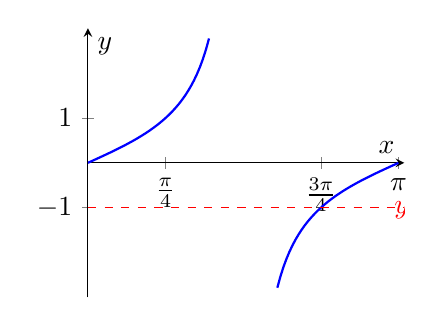
\begin{tikzpicture}
\begin{axis}[
    width=5.6cm, height=5cm,
    axis lines=middle,
    xlabel={$x$}, ylabel={$y$},
    xmin=0, xmax=3.2, ymin=-3, ymax=3,
    xtick={0,0.785,2.356,3.14},
    xticklabels={$0$,$\frac\pi4$,$\frac{3\pi}{4}$,$\pi$},
    ytick={-1,1},
    restrict y to domain=-3:3,
]
\addplot[thick,blue,domain=0:1.5,samples=50] {tan(deg(x))};
\addplot[thick,blue,domain=1.64:3.14,samples=50] {tan(deg(x))};
\addplot[dashed,red] coordinates {(0,-1)(3.2,-1)};
\node[red,right] at (axis cs:3.0,-1) {$y=-1$};
\end{axis}
\end{tikzpicture}
\end{column}
\end{columns}
\end{frame}

% ---------- 第2题 ----------
\begin{frame}[t]{练习三 2：写 $x$ 的范围}
\textbf{2.} 观察正切曲线，写出满足下列条件的 $x$ 值的范围：
\begin{enumerate}[(1)]
  \item $\tan x>0$； \qquad
  \item $\tan x=0$； \qquad
  \item $\tan x<0$。
\end{enumerate}
\end{frame}

\begin{frame}[t]{练习三 2 解答}
\begin{tcolorbox}[colback=orange!10,colframe=orange,title=\textbf{解（$k\in\mathbf Z$）}]
\begin{enumerate}[(1)]
  \item $\tan x>0$：\alert{$\left(k\pi,\,\dfrac{\pi}{2}+k\pi\right)$}；
  \item $\tan x=0$：\alert{$x=k\pi$}；
  \item $\tan x<0$：\alert{$\left(-\dfrac{\pi}{2}+k\pi,\,k\pi\right)$}。
\end{enumerate}
\small（正切在每个周期内单调递增，与 $x$ 轴交点为 $k\pi$，渐近线为 $x=\dfrac{\pi}{2}+k\pi$。）
\end{tcolorbox}
\end{frame}

% ---------- 第3题 ----------
\begin{frame}[t]{练习三 3：求定义域}
\textbf{3.} 求函数 $y=\tan 3x$ 的定义域。
\end{frame}

\begin{frame}[t]{练习三 3 解答}
\begin{tcolorbox}[colback=orange!10,colframe=orange,title=\textbf{解}]
正切函数要求角的终边不在 $y$ 轴上，即
\[
3x\ne\frac{\pi}{2}+k\pi,\quad k\in\mathbf Z.
\]
解得
\[
x\ne\frac{\pi}{6}+\frac{k\pi}{3},\quad k\in\mathbf Z.
\]
故定义域为
\[
\alert{\left\{x\,\middle|\,x\ne\frac{\pi}{6}+\frac{k\pi}{3},\ k\in\mathbf Z\right\}}.
\]
\end{tcolorbox}
\end{frame}

% ---------- 第4题 ----------
\begin{frame}[t]{练习三 4：求周期}
\textbf{4.} 求下列函数的周期：
\begin{enumerate}[(1)]
  \item $y=\tan 2x$，$x\ne\dfrac{\pi}{4}+\dfrac{k\pi}{2}\ (k\in\mathbf Z)$； \qquad
  \item $y=5\tan\dfrac{x}{2}$，$x\ne(2k+1)\pi\ (k\in\mathbf Z)$。
\end{enumerate}
\end{frame}

\begin{frame}[t]{练习三 4 解答}
\begin{tcolorbox}[colback=orange!10,colframe=orange,title=\textbf{解}]
$y=A\tan(\omega x+\varphi)$ 的周期为 $T=\dfrac{\pi}{|\omega|}$。
\vspace{0.3em}
(1) $\omega=2$，故 $T=\dfrac{\pi}{2}$，即周期为 \alert{$\dfrac{\pi}{2}$}；
\vspace{0.3em}
(2) $\omega=\dfrac12$，故 $T=\dfrac{\pi}{1/2}=2\pi$，即周期为 \alert{$2\pi$}。
\end{tcolorbox}
\end{frame}

% ---------- 第5题 ----------
\begin{frame}[t]{练习三 5：比较正切值大小}
\textbf{5.} 不通过求值，比较下列各组中两个正切值的大小：
\begin{enumerate}[(1)]
  \item $\tan(-52^\circ)$ 与 $\tan(-47^\circ)$； \qquad
  \item $\tan\dfrac{13\pi}{4}$ 与 $\tan\dfrac{17\pi}{5}$。
\end{enumerate}
\end{frame}

\begin{frame}[t]{练习三 5 解答}
\begin{tcolorbox}[colback=orange!10,colframe=orange,title=\textbf{解}]
(1) $-52^\circ,-47^\circ\in\left(-90^\circ,90^\circ\right)$，$y=\tan x$ 在此区间单调递增。
\[\because -52^\circ<-47^\circ,\quad\therefore \tan(-52^\circ)\alert{<}\tan(-47^\circ).
\]
(2) 化简：
\[
\tan\frac{13\pi}{4}=\tan\!\left(3\pi+\frac{\pi}{4}\right)=\tan\frac{\pi}{4},
\]
\[
\tan\frac{17\pi}{5}=\tan\!\left(2\pi+\frac{7\pi}{5}\right)=\tan\!\left(\pi+\frac{2\pi}{5}\right)=\tan\frac{2\pi}{5}.
\]
在 $\left(0,\dfrac{\pi}{2}\right)$ 上 $\tan x$ 单调递增，$\dfrac{\pi}{4}<\dfrac{2\pi}{5}$，故
\[
\tan\frac{13\pi}{4}\alert{<}\tan\frac{17\pi}{5}.
\]
\end{tcolorbox}
\end{frame}

\begin{frame}[c]
  \begin{center}
    {\Huge\calligra Thanks!}
  \end{center}
\end{frame}

\end{document}
